%************************************************
\chapter{Symbolic Representation}
\label{chapter:symbolic_representation}
%************************************************

\section{Representing Reflective Thinking Activity}

Reflective thinking exists as dynamic activities in Duration alongside
the physical activities that have just been described.  I will refer
to the subgraph of the simulation state, $S$, that represents the
$\text{reflective}^1$ thinking activities as $\mathcal{R}^1$.  The
first symbolic references to reflective thinking are now introduced to
this layer of the model.  Note that I have not introduced any specific
symbolic physical activity to the model.  The block example is just
that, an example.  Having the reflective focus be undescribed is
important because then the focus is not restricted, which allows a
recursive application of reflection to itself, whatever the specific
graph representation described.  This is a key point because the
general model of reflection applying to \emph{any} given labelled
graph means that it allows for this recursive definition of layered
reflective thinking.

\section{Physical Activity is Any Prior Existing Graph}

The graph of physical activities must necessarily exist prior to
reflectively thinking about it.  Because this prior activity is
defined to be \emph{any} graph, what remains in order to build $n$
layers of reflective thinking activity is to define planning activity
that reflects upon this prior activity.  Therefore, subsequently, no
matter what the reflective thinking description, this reflective
thinking activity can be duplicated in $n$ reflective layers that will
think about any given graph representation of activity.  Allowing the
physical activity to a be an undescribed graph is important in order
to allow this recursion.  Notice that the physical activity is not
necessarily composed of anything resembling objects, since graphs are
a general representation that could just as easily represent one
single number line, or even an infinitely finely interpolated
multidimensional Space.  If some prior physical activity can be
represented as a graph, then this simulation of reflective thinking is
applicable.

\section{Defining N Layers of Reflective Thinking Activities}

Layers of reflective activity are defined inductively, beginning with
$\text{reflective}^0$ layer of activity, $\mathcal{R}^0$, as the
initial given physical activity.  Then, each subsequent layer of
$\text{reflective}^{n+1}$ thinking activity, $\mathcal{R}^{n+1}$, is
defined in terms of $\mathcal{R}^n$ in
{\mbox{Equations~\ref{equation:define_reflective_n_activity_graph_first}}}
{\mbox{through~\ref{equation:define_reflective_n_activity_graph_last}}}.
\begin{align}
\label{equation:define_reflective_n_activity_graph_first}
                                        \mathcal{R}^0 &\equiv \text{\emph{Physical Layer of Activities}} \\
                                   \mathcal{R}^{n+1}_V &\subset S_V \setminus \bigcup_{k=0}^n\mathcal{R}^k_V \\
                                   \mathcal{R}^{n+1}_E &= (\mathcal{R}^{n+1}_V \times \mathcal{R}^{n+1}_V) \cap S_E \\
                              \mathcal{R}^{n+1}_\mu(v) &= {\left\{
                                                            \begin{array}{ll}
                                                              S_\mu(v)         & \text{if }v {\in} \mathcal{R}^{n+1}_V \\
                                                              \text{undefined} & \text{otherwise}
                                                            \end{array}
                                                          \right.} \\
\label{equation:define_reflective_n_activity_graph_last}
                              \mathcal{R}^{n+1}_\nu(e) &= {\left\{
                                                            \begin{array}{ll}
                                                              S_\nu(e)          & \text{if }e {\in} \mathcal{R}^{n+1}_E \\
                                                              \text{undefined} & \text{otherwise}
                                                            \end{array}
                                                          \right.}
\end{align}
Note that there can be edges between activities in subsequent layers.
These edges are not within any of the graphs of the reflective layers
of thinking, but they do exist in the state graph, $S$.  The edges
that relate the reflective layers of activity in the simulation model
are a necessary component of dynamic symbolic references to activities
in the layers below the symbolic activity.  In other words,
$\bigcup_{k=0}^\infty\mathcal{R}^k\ \subset\ S$, the simulation state
is greater than the union of its reflective layers.

\section{Representing Static Symbols}

In order to describe symbolization, a representation for a simulated
symbol must be defined.  A symbol is the most interesting object in
the model because it functions as a static reference to the dynamic,
while being fundamentally dynamic itself.  There are two primary
features of a symbolic reference:
\begin{itemize}
\item A symbol functions as a static reference and, thus, can be
  ordered in Spatial arrangements that function as static orderings.
\item A symbol is fundamentally dynamic and, thus, exists as dynamic
  activities in a referential dynamic continuous Spatial relationship
  with other dynamic activities in Duration.
\end{itemize}
A symbol is actively maintained in Duration, so the existence of a
simulated symbol in the simulation model would need to be added to the
set of all simulated activities in Duration.  The set of symbols* in
layer $n$ is defined to be $X^{n*}$.
{\mbox{Equations~\ref{equation:define_symbol_first}}}
{\mbox{and~\ref{equation:define_symbol_last}}} define layered sets of
symbols*:
\begin{align}
\label{equation:define_symbol_first}
           X^{n*} &= \left\{x^* : \begin{array}{l}
                                   x^* \in \mathcal{R}^n_V ~\wedge~ \\
                                   ~~\left(\forall_{v \in \mathcal{R}^n_V}, \begin{array}{l}
                                                                          S_\mu(v) = \text{\tt{Reflective}} \rightarrow \\
                                                                          ~~x^* \in v.\text{\tt{symbol}}
                                                                        \end{array}\right)
                                 \end{array}\right\} \\
\label{equation:define_symbol_last}
           x^{n*} &\in X^{n*}
\end{align}

\section{Representing Symbolic Reference}

Because dynamic activities in Duration cannot be ordered in Space by
the reflective thinking layers, the most important aspect of the
reflective simulation is the capability to create a static reference,
$x^*$, which has an associated dynamic representation of an arbitrary
subgraph of activity, $\Psi(x^*)$.  Note that while $\Psi(x^*)$
represents a potential subgraph of the simulation state, this subgraph
may or may not actually exist in the simulation state, $S$.  This
symbolic representative capability is the basis of symbolic perception
and memory.

Because the simulation state is a static symbolic representation of
the actual dynamic activities in Duration, simulation of the dynamic
reflective representation must also be in the same simulated terms of
dynamic physical activities.  Considering this dynamic activity to be
symbolic helps in explaining the relationship between the dynamic and
the static, as long as the distinction is kept clear and the
simulation of the dynamic is not confused with the simulation of the
static.  The confusion would arise because both are modelled as
symbols in the state graph, $S$, of the simulation model.  Of course,
in actuality, the dynamic physical activities do not have symbolic
terms.  I will continue to use the asterisk (*) notation when
referring to the simulation of actively static symbolic references as
opposed to the simulation of the otherwise purely dynamic activities
in Duration.
{\mbox{Equations~\ref{equation:first_order_reflection_representation_in_state_first}}}
{\mbox{through~\ref{equation:first_order_reflection_representation_in_state_last}}}
show a definition of a static symbolic reference, $x^*$, to a dynamic
reflective representation of a subgraph of activity, $\Psi(x^*)$, not
necessarily actually within the state graph, $S$.
\begin{align}
\label{equation:first_order_reflection_representation_in_state_first}
                                                   \forall_{v \in \Psi_V(x^*)}, ~v &\in x^*.\text{\tt{node}} \\
                                 \forall_{v \in \Psi_V(x^*)}, ~v.\text{\tt{label}} &= \{\Psi_\mu(x^*)(v)\} \\
                                                   \forall_{e \in \Psi_E(x^*)}, ~e &\in x^*.\text{\tt{edge}} \\
     \forall_{e \in \Psi_E(x^*)}, ~[e = (e_{v_1}, e_{v_2}) \wedge e.\text{\tt{tail}} &= \{e_{v_1}\}] \\
     \forall_{e \in \Psi_E(x^*)}, ~[e = (e_{v_1}, e_{v_2}) \wedge e.\text{\tt{head}} &= \{e_{v_2}\}] \\
\label{equation:first_order_reflection_representation_in_state_last}
                                 \forall_{e \in \Psi_E(x^*)}, ~e.\text{\tt{label}} &= \{\Psi_\nu(x^*)(e)\}
\end{align}
{\mbox{\autoref{figure:simulation_reflective_1_example_state}}} shows
an example of the representation for a symbolic reference to the
$\text{reflective}^0$ layer in the $\text{reflective}^1$ layer.
\begin{figure}
\center
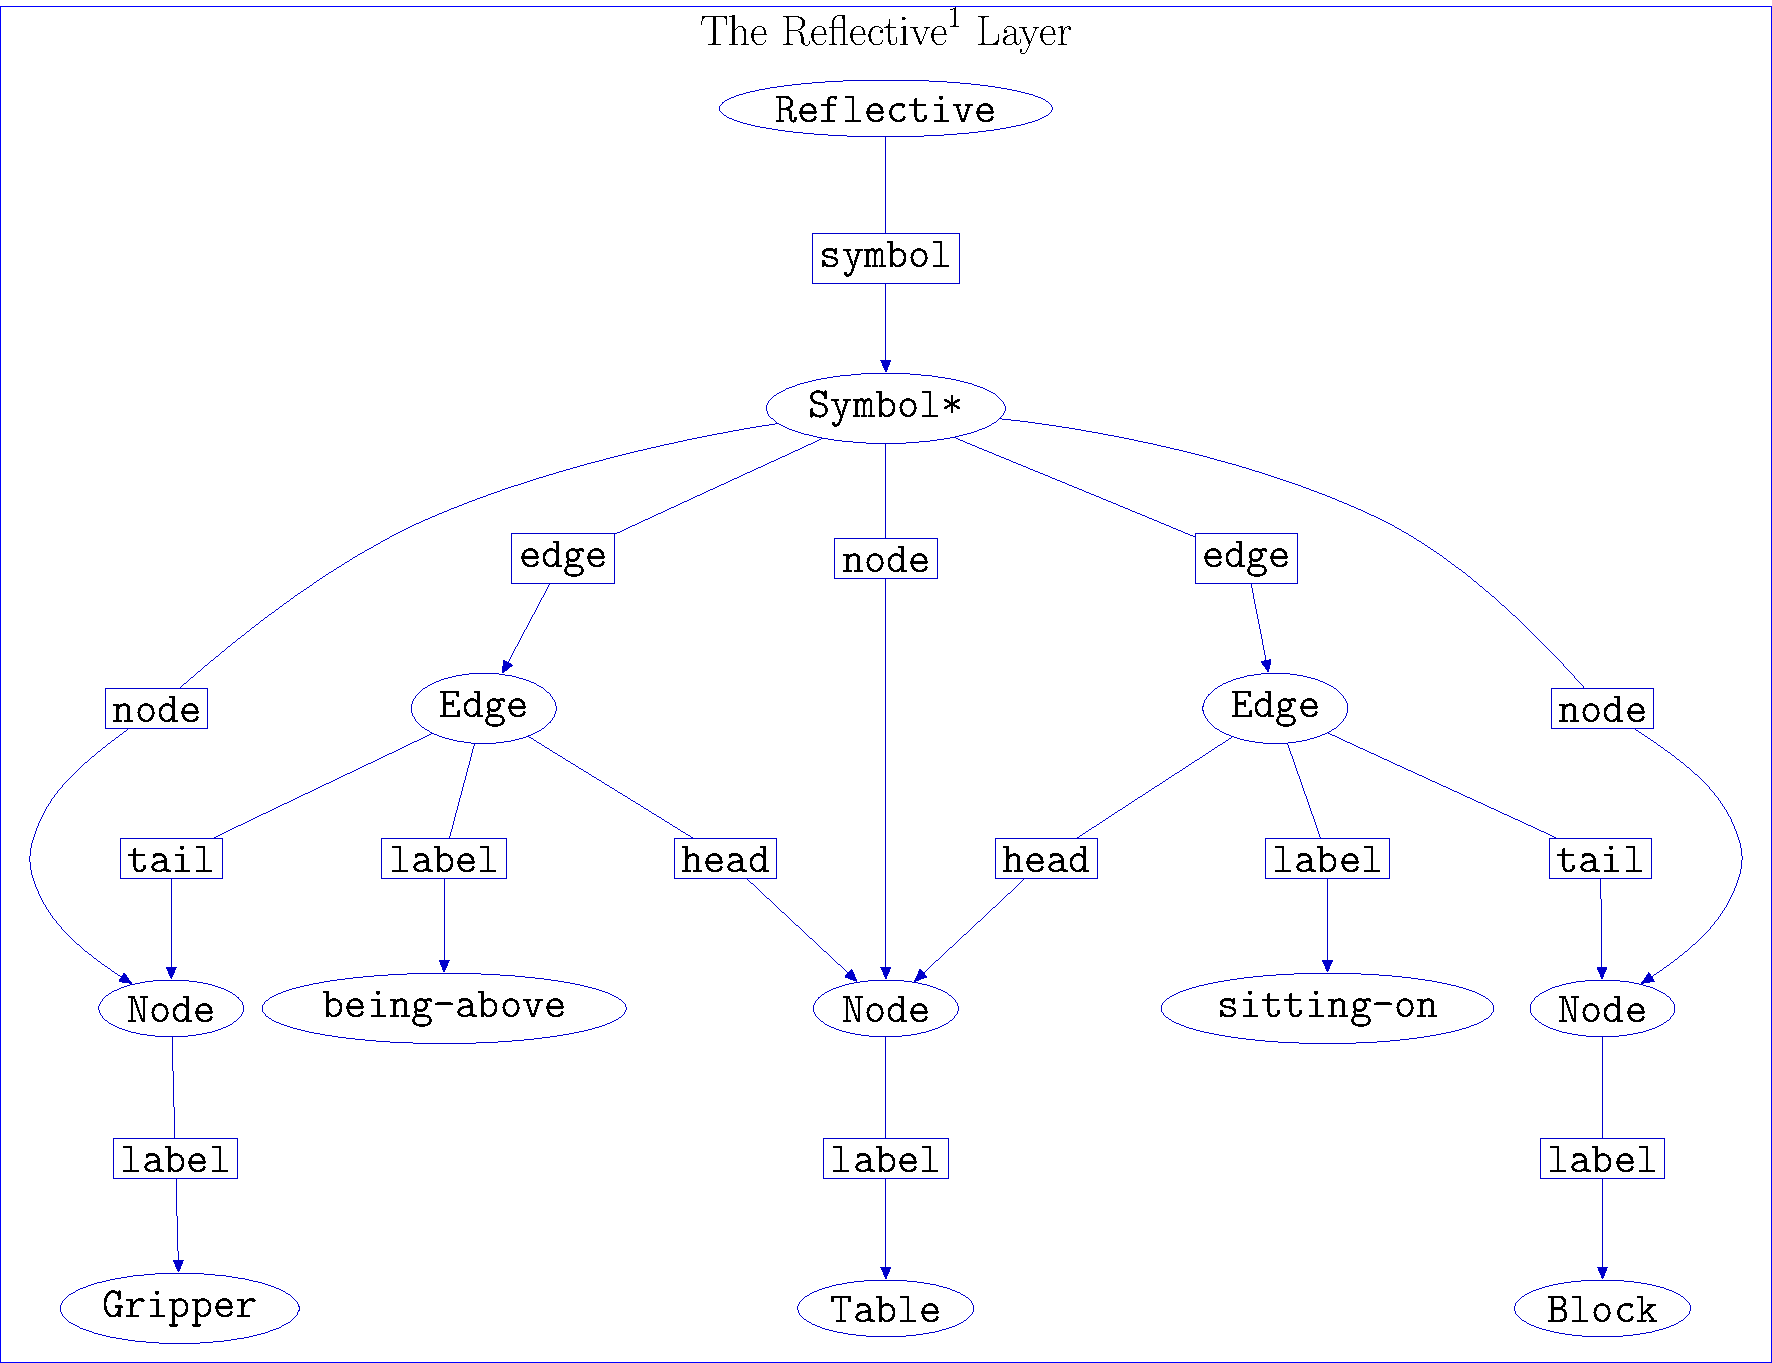
\includegraphics[width=12cm]{gfx/simulation_reflective_1_example_state}
\caption[An example of the representation for symbolic reference.]{An
  example of the representation for symbolic reference, where the
  dynamic referent is the physical activity of a block being on a
  table in conjunction with a gripper being above the same table.}
\label{figure:simulation_reflective_1_example_state}
\end{figure}

\section{A Visualization of a Reflective Relationship}

When reflective graph structures, as in
{\mbox{\autoref{figure:simulation_reflective_1_example_state}}}, get
to be larger, they can be confusing when shown in full structural
detail.  In order to simplify the visual representation of a
reflective relationship, I will sometimes use a trapezoidal edge-like
visual in order to present the same complicated relationship structure
in a simpler way.
{\mbox{\autoref{figure:reflective_relationship_visualization}}} shows
a simpler visualization of the same example reflective relationship.
\begin{figure}
\center
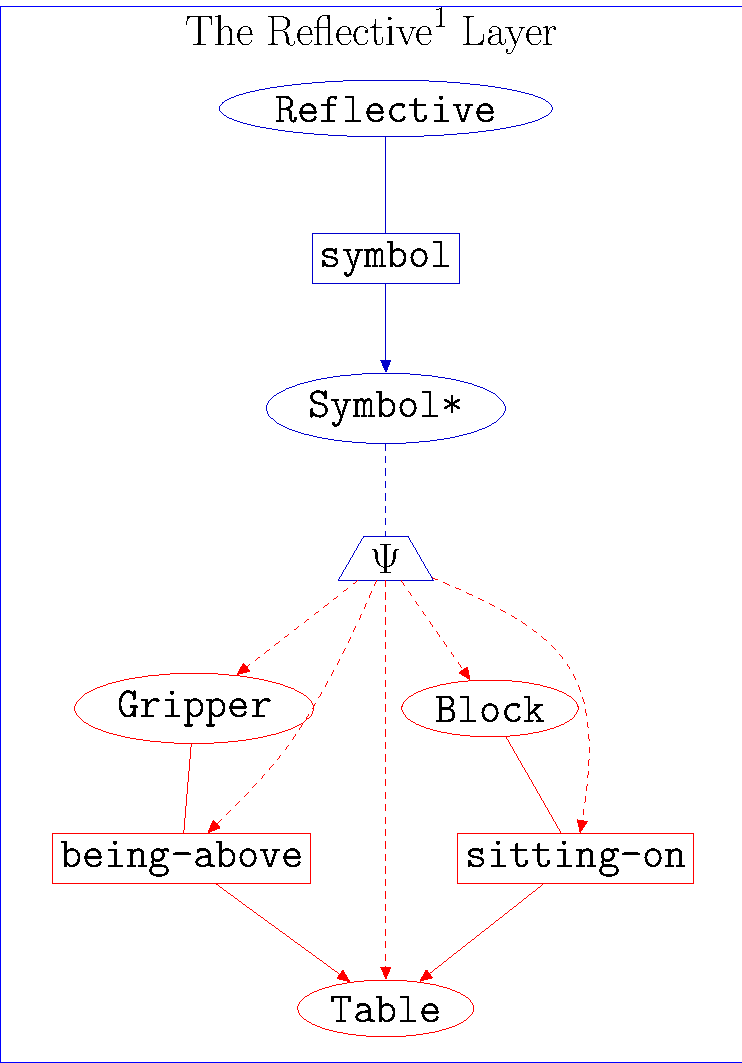
\includegraphics[width=6cm]{gfx/reflective_relationship_visualization}
\caption[A shorthand visualization for a symbolic reference.]{A
  shorthand visualization for a symbolic reference, where the
  trapezoid is a shorthand, for the same representation depicted in
  {\mbox{\autoref{figure:simulation_reflective_1_example_state}}}.
  The symbolic referent subgraph is pictured in red because this
  subgraph does not actually exist in the simulation state graph, $S$.
  Instead, the symbolic referent subgraph's \emph{representation}
  actually dynamically exists in the simulation state graph,
  $S$. Thus, the symbolic representation operator, $\Psi$, is not a
  symbol in the state graph, $S$, but represents the relationship to
  the representation of the non-existent subgraph that appears in
  red.}
\label{figure:reflective_relationship_visualization}
\end{figure}

\section{Representing Symbolic Perception and Memory}

{\mbox{\autoref{figure:example_symbolic_reference_to_physical_activity}}}
shows an example of a symbol*, $x^*$, in the first-order reflective
layer.  Notice that $\Psi(x^*)$ is isomorphic to a subgraph of the
$\text{reflective}^0$ layer, $\mathcal{R}^0$.  When a symbolic
representation is isomorphic to a subgraph of the layers below it, the
symbol is said to be a {\emph{symbolic perception}}, or simply, a
{\emph{percept}}.
{\mbox{\autoref{equation:definition_of_symbolic_percept}}} defines
when a symbolic referent is considered a percept based on its
isomorphic relationship with layers of activity below it:
\begin{equation}
\label{equation:definition_of_symbolic_percept}
\text{percept}^n(x^*) = \left\{\begin{array}{ll}
                                 \begin{array}{l}
                                   \text{\emph{True}} \\
                                   \text{~~}
                                 \end{array} & \begin{array}{l}
                                                 \text{if } \Psi(x^*) \text{ is isomorphic to a} \\
                                                 \text{~~subgraph of } S \setminus \bigcup_{k=n}^\infty{\mathcal{R}^k}
                                               \end{array} \\
                                 \begin{array}{l}
                                   \text{\emph{False}}
                                 \end{array} & \text{otherwise}
                               \end{array}\right.
\end{equation}
{\mbox{\autoref{figure:example_symbolic_memory}}} shows a symbolic
reflective reference to the physical layer of activity that is not
perceived because it is not isomorphic to any subgraph in the
$\text{reflective}^0$ layer, $\mathcal{R}^0$.  When a symbol is not
isomorphic to a subgraph in the layers below it, this is referred to
as a \emph{symbolic memory}.
\begin{figure}
\center
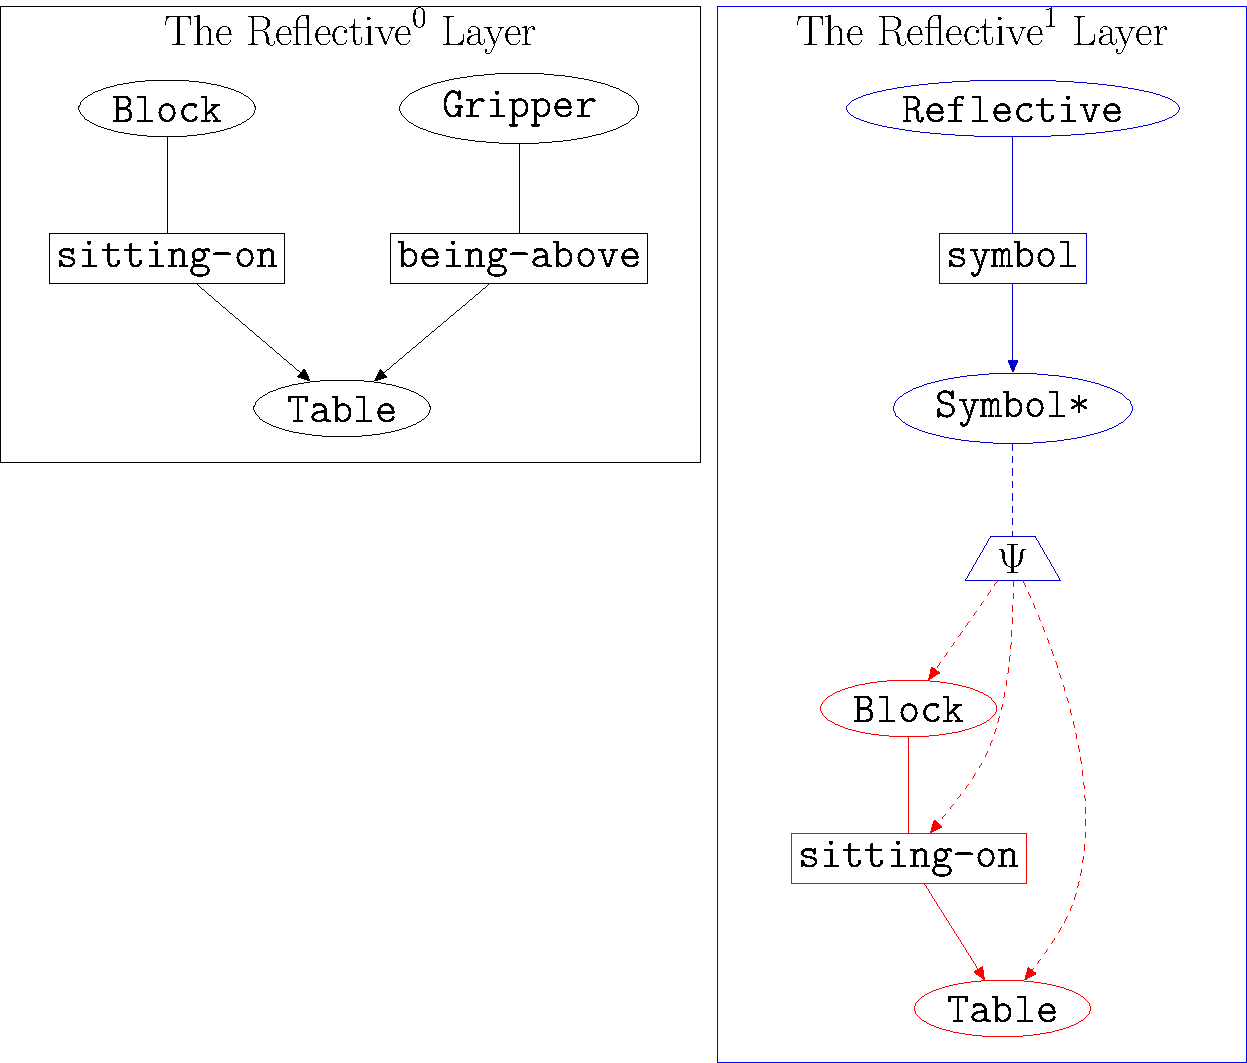
\includegraphics[height=8cm]{gfx/example_symbolic_reference_to_physical_activity}
\caption[Example of a perceived first-order symbolic reference to the
  physical layer of activity.]{Example of a perceived first-order
  symbolic reference to the physical layer of activity,
  i.e. $\Psi(x^*)$ is isomorphic to a subgraph of $\mathcal{R}^0$.}
\label{figure:example_symbolic_reference_to_physical_activity}
\end{figure}
\begin{figure}
\center
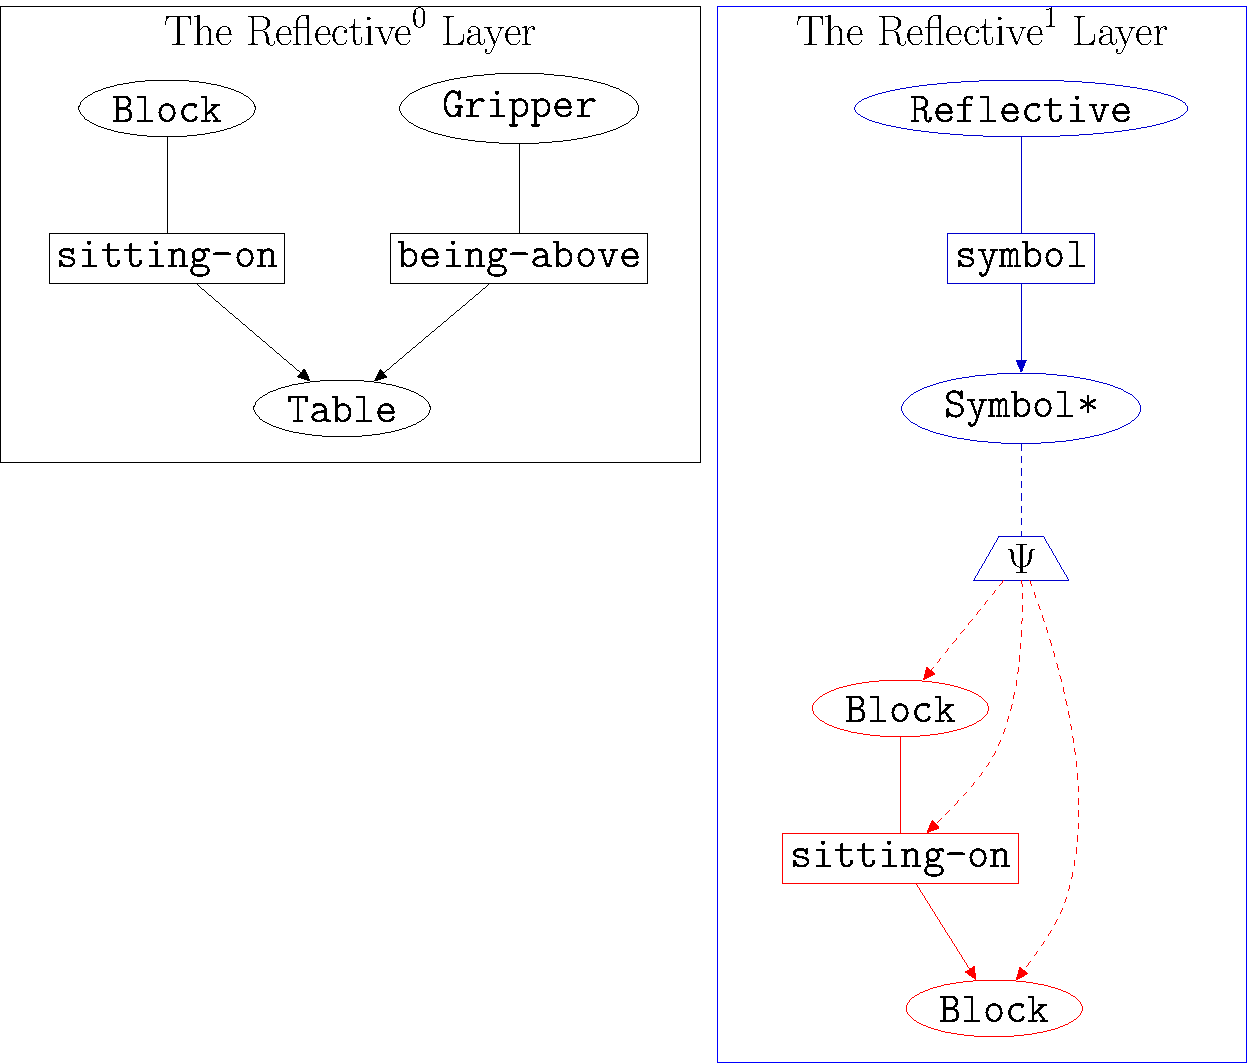
\includegraphics[height=8cm]{gfx/example_symbolic_memory}
\caption[Example of a non-perceived symbol, or symbolic
  memory.]{Example of a non-perceived symbol, or symbolic memory,
  $x^*$, i.e. $\Psi(x^*)$ is not isomorphic to a subgraph of
  $\mathcal{R}^0$.}
\label{figure:example_symbolic_memory}
\end{figure}

\section{Second-order Symbolic Representation}

The second-order layer of reflective thinking is the first layer that
can reflect on the existence of the symbols of the first-order
reflective layer.
{\mbox{\autoref{figure:example_second_order_symbol}}} shows an example
of a second-order symbolic reference to a first-order symbolic
representation.
\begin{figure}
\center
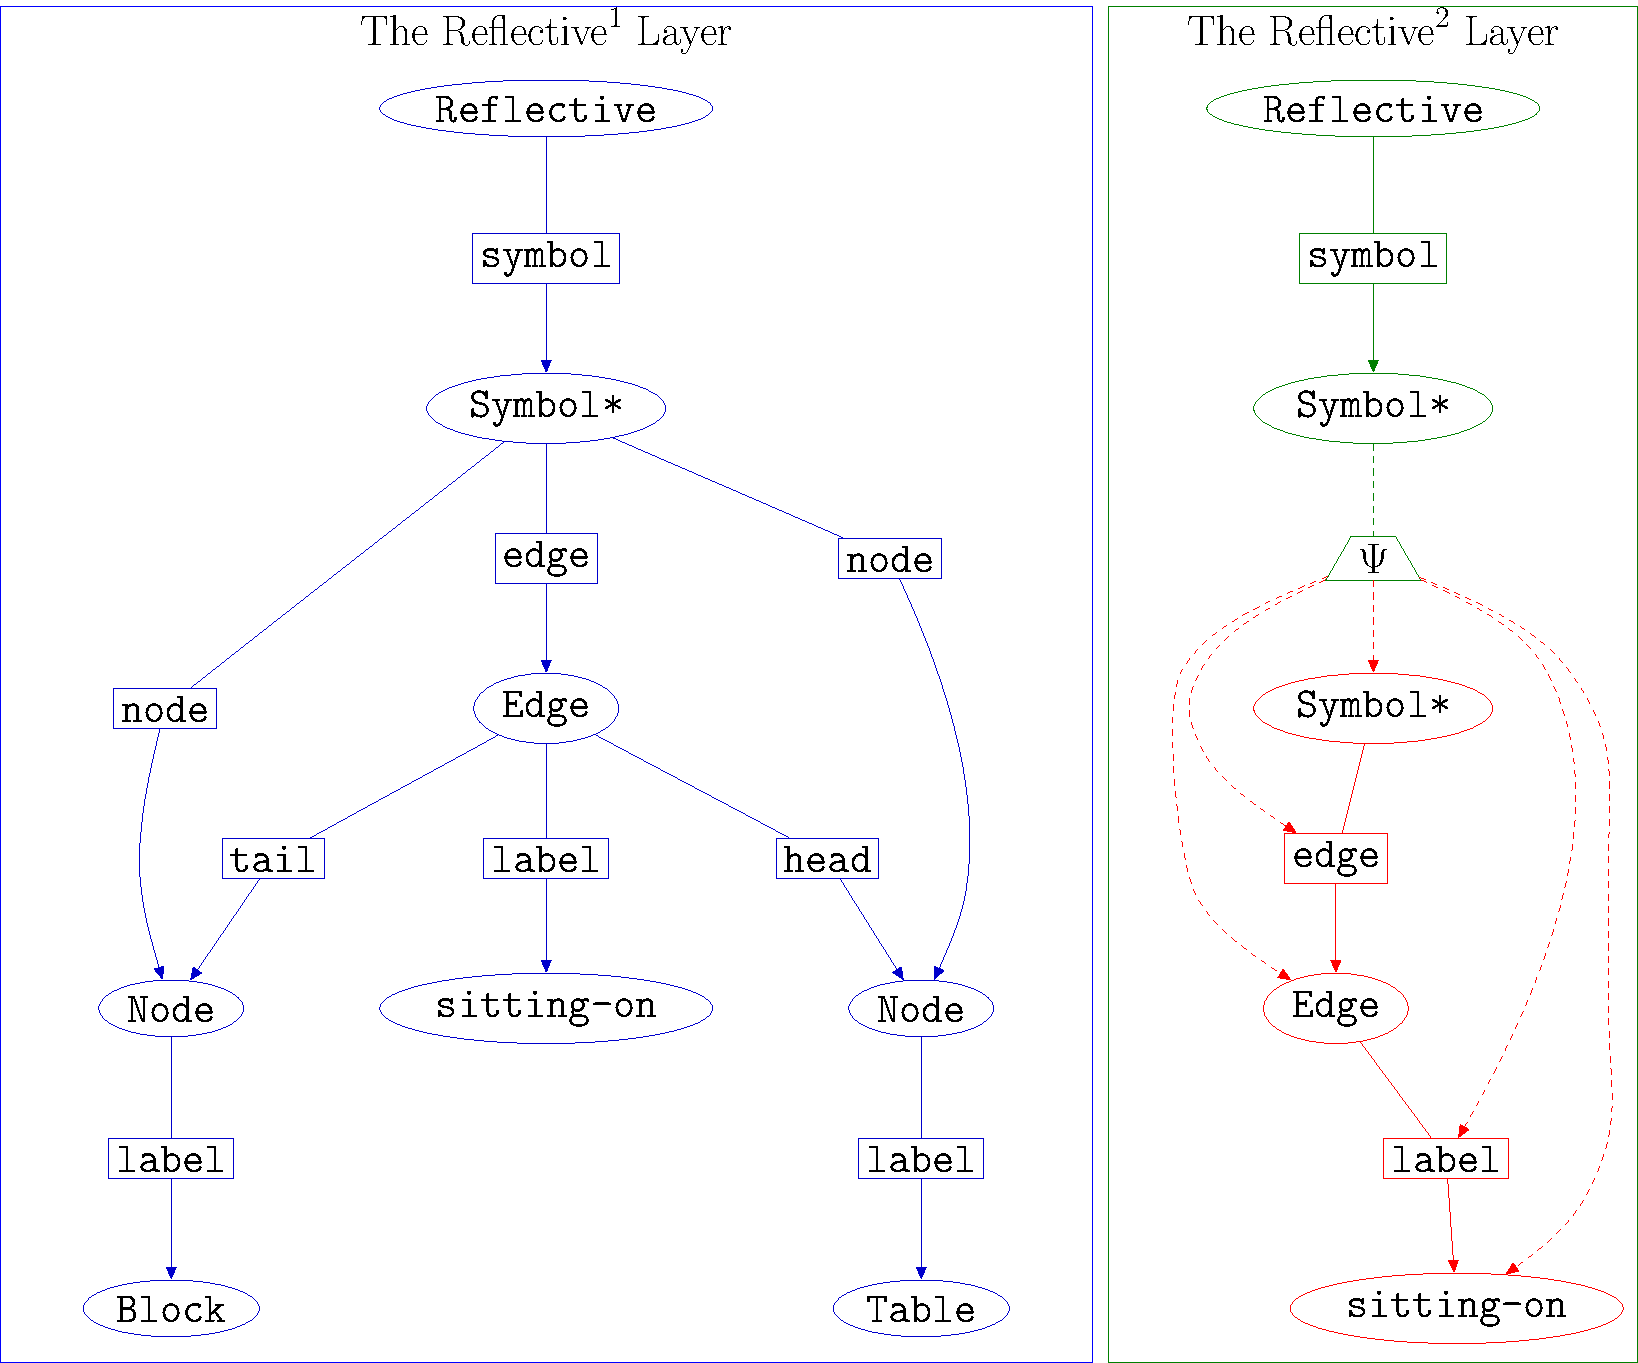
\includegraphics[width=12cm]{gfx/example_second_order_symbol}
\caption[Example of a second-order symbol representing first-order
  symbolization activity.]{Example of a second-order symbol
  representing an aspect of first-order symbolization.  Note that the
  actually existent symbolic representation in the first-order
  reflective layer is shown in full detail, while the red subgraph in
  the second-order symbolic representation is short-hand for the much
  more complex actually existent activity in this layer.}
\label{figure:example_second_order_symbol}
\end{figure}
